%%%%% SOME OPTIONS %%%%% 
\newcommand{\german}{false} % germanTrue or false --> Switch between german and english headers / titlepage
\newcommand{\coloredTitlePage}{true} % Switch between colored and BW titlepage
\newcommand{\company}{false}
\newcommand{\ECE}{true}
%%%%% Required Settings for the template %%%%%
%%%%% Configuration Package for the ThesisTemplate ECE / AEE %%%%%%
%
% Created by Mayer Florian October/2016
% v1.0

%======= DocumentClass ===========%
\documentclass[11pt, openright]{book} %Extarticle supports more FontSizes

%========= ADD Latex PACKAGES =========%
\usepackage{tabularx}         
\usepackage{parskip}%NEW
\newcolumntype{x}[1]{!{\centering\arraybackslash\vrule width #1}}
\usepackage{booktabs}
\usepackage[utf8]{inputenc} %to allow vowel mutations
\usepackage{tikz} % Schematic creator with TikZ in LaTex
\usepackage{geometry,titlesec,layout}
\usepackage{subfigure}
\usepackage{xcolor,colortbl}
%\usepackage{graphicx,rotating}
\usepackage{float}
\usepackage{epstopdf}
\usepackage[titles]{tocloft}
\usepackage{blindtext}
\usepackage{anyfontsize}
\usepackage{setspace,varwidth}
\usepackage{ifthen}
\usepackage{multicol,multirow}
\usepackage{makecell}
\usepackage[stable,bottom,hang,splitrule,multiple]{footmisc}% customize footnotes
\usepackage[final]{listings}% program code listings
\usepackage[%
headtopline,plainheadtopline,% activate all lines (header and footer)
headsepline,plainheadsepline,%
footsepline,plainfootsepline,%
footbotline,plainfootbotline,%
nouppercase% auto update \..mark
]{scrlayer-scrpage}% (KOMA)

\usepackage[%
breaklinks=true,% allow line break in links
colorlinks=true,% if false: framed link
linkcolor=black,anchorcolor=black,citecolor=black,filecolor=black,%
menucolor=black,urlcolor=black]{hyperref}% hyperlinks for references

\usepackage{amssymb}
\usepackage{emptypage}
\usepackage{glossaries}
\usepackage{appendix}
\usepackage{mdframed}
\usepackage{etoolbox}
\usepackage{chngcntr} 

\usepackage{textcomp}
\usepackage{lmodern}
\usepackage[european, straightvoltages, americaninductors, oldvoltagedirection]{circuitikz}

%========= ADD TikZ PACKAGES =========%
\usetikzlibrary{matrix,calc,positioning,arrows,shapes}
\usetikzlibrary{decorations.pathreplacing}

%======= END ADD PACKAGES =======%
\geometry{a4paper,twoside,%
	%textheight=205mm, %246mm,%
	textwidth=160mm,%
	top = 3cm,
	bottom = 4.5cm,
	heightrounded=false,% round textheight to multiple of lines (avoids overfull vboxes)
	ignoreall=true,% do not include header, footer, and margins in calculations
	marginparsep=5pt,% marginpar only used for signs (centered), thus only small sep. needed
	marginparwidth=10mm,% prevent margin notes to be out of page
	hmarginratio=1:2,
	voffset = 2.25mm,
	%headheight = 16mm,
	headsep = 9mm,
	footskip = 13mm
}
\linespread{1.4}
%======= DEFINE COLORS ===========%
\definecolor{DENcol}{RGB}{35,171,196} % Department Colour


%======= Re-Define Essential Commands and store old ones ======%
\newcommand{\ChapterFont}{qag}
\newcommand{\WorkingFont}{\rmdefault}
\renewcommand{\familydefault}{\WorkingFont}
\normalfont

%======= Set Depths of TOC / TOF / TOL =======%

\renewcommand{\cftchapfont}{\bf\large\fontfamily{\sfdefault}\selectfont}
\renewcommand{\cftpartfont}{\bf\large\fontfamily{\sfdefault}\selectfont}

\ifthenelse{\equal{\german}{true}}
{
\usepackage[ngerman]{babel}
\renewcommand{\lstlistingname}{Programmcode} 
}
%====== Usefull Additional Commands =======%

% Make clickable footnote
    \newcommand{\hyperfootnote}[1][]{\def\ArgI\hyperfootnoteRelay}
    % relay to new command to make extra optional command possible
    \newcommand\hyperfootnoteRelay[2][]{\href{#1#2}{\ArgI}\footnote{\href{#1#2}{#2}}}
    % the first optional argument is now in \ArgI, the second is in #1
    %http://www.brechtdeman.com/blog/latex-clickable-footnote.html
    % Simple (no arguments)
    %    \hyperfootnote{http://www.mywebsite.com}
    % Link text (1 argument)
    %   \hyperfootnote[My website]{http://www.mywebsite.com}
    % Link text and invisible prefix (2 arguments)
    %   \hyperfootnote[My website][http://]{www.mywebsite.com}

\newcommand{\ie}{i.\,e.}
\newcommand{\Ie}{I.\,e.}
\newcommand{\eg}{e.\,g.}
\newcommand{\Eg}{E.\,g.} 

%====== Heading Commands =======%

\pagestyle{scrheadings}%
% \setlength\parindent{0cm}% no indentation for first line of new paragraph
% \raggedbottom% do not try to fill pages

% header and footer size
\setheadwidth{text}% set header width to textwidth
\setfootwidth{text}% set footer width to textwidth
\setheadtopline[textwithmarginpar]{0.25pt}% set up separator lines (greater width than text)
\setheadsepline[textwithmarginpar]{0.25pt}
\setfootsepline[textwithmarginpar]{0.25pt}
\setfootbotline[textwithmarginpar]{0.25pt}

\renewcommand*\chaptermark[1]{\markleft{\thechapter~#1}}
\renewcommand*\sectionmark[1]{\markright{\thesection~#1}} 

\clearscrheadfoot % clear everything
\ihead[]{}%
\ohead[\ShortTitle]{\footnotesize\headmark}%
%\cfoot[\footnotesize\ConfidNote]{\footnotesize\ConfidNote}%

\ofoot[\ifthenelse{\equal{\thepage}{}}{\pagemark}{--~~\pagemark~~--}]{\ifthenelse{\equal{\thepage}{}}{\pagemark}{--~~\pagemark~~--}}%

%============== Chapter / Section / Subsection Style ==== %
\titleformat{\part}[display]
   {\fontfamily{\sfdefault}\bfseries\fontsize{26}{26}\selectfont\filcenter}
   {\fontfamily{\sfdefault}\bfseries\fontsize{30}{22}\selectfont\partname{} \thepart}
   {0.5em}
   {}

\titleformat{\chapter}[display]
{\fontfamily{\sfdefault}\bfseries\fontsize{22}{22}\selectfont}%\
{
\begin{tikzpicture}[overlay]
	\node (CoolTitle) at (12,1) [opacity=0.325]{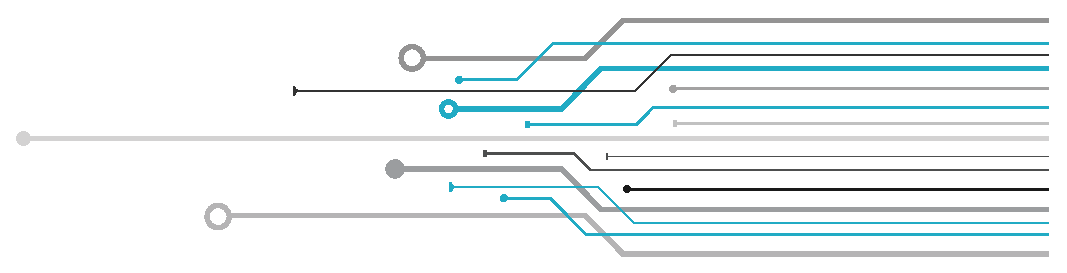
\includegraphics[scale=0.75]{temp_graphics/chapterBacking.eps}};
	\node (titleNumber) at ($(CoolTitle)+(3,0)$) {\textcolor{black!80}{\fontfamily{\ChapterFont}\bfseries\Large\fontsize{80}{80}\selectfont\thechapter}};
\end{tikzpicture}
}
{0.05em}%
{\vspace{0.25ex}\filleft}%

\titleformat{\section}{\Large \bfseries \sffamily}{\thesection}{1 em}{}
\titleformat{\subsection}{\large \bf \sffamily}{\thesubsection}{1 em}{}
\titleformat{\subsubsection}{\large \bf \sffamily}{\thesubsubsection}{1 em}{}

%%%% CLEAR DOUBLE-PAGE
% redefine cleardoublepage...
\makeatletter
\renewcommand{\cleardoublepage}{\clearpage\if@twoside\ifodd\c@page\else\thispagestyle{plain}\hbox{}\newpage\if@twocolumn\hbox{}\newpage\fi\fi\fi}
% ...and define empty double page (e.g., for title sheet)
\newcommand{\emptydoublepage}{\clearpage\if@twoside\ifodd\c@page\else\thispagestyle{empty}\hbox{}\newpage\if@twocolumn\hbox{}\newpage\fi\fi\fi}%
% ...and also an empty single page
\newcommand{\emptypage}{\clearpage\thispagestyle{empty}\hbox{}\newpage\if@twocolumn\hbox{}\newpage\fi}%
\makeatother

%%%%% Correct Even and Odd Pages %%%%%
\let\tmp\oddsidemargin
\let\oddsidemargin\evensidemargin
\let\evensidemargin\tmp
\reversemarginpar

% code listings
\lstloadlanguages{Bash,VHDL,Matlab,[ANSI]C,Java,[LaTeX]TeX}

\lstset{
	frame=top,frame=bottom,
	basicstyle=\fontsize{8}{8}\normalfont\sffamily,    % the size of the fonts that are used for the code
	stepnumber=1,                           % the step between two line-numbers. If it is 1 each line will be numbered
	numbersep=6pt,                         % how far the line-numbers are from the code
	tabsize=2,                              % tab size in blank spaces
	extendedchars=true,                     %
	breaklines=true,                        % sets automatic line breaking
	captionpos=t,                           % sets the caption-position to top
	mathescape=true,
	stringstyle=\color{black}\ttfamily, % Farbe der String
	showspaces=false,           % Leerzeichen anzeigen ?
	showtabs=false,             % Tabs anzeigen ?
	xleftmargin=15pt,
	framexleftmargin=14pt,
	framexrightmargin=9pt,
	framexbottommargin=5pt,
	framextopmargin=5pt,
	showstringspaces=false,      % Leerzeichen in Strings anzeigen ?
	numbers = left,
	linewidth = 150mm
}
%%%% MDBOX Setup
\mdfsetup{%
middlelinecolor=red,
middlelinewidth=2pt,
backgroundcolor=DENcol!10,
roundcorner=10pt,
topline = false,
bottomline = false,
rightline = false,
linecolor = DENcol,
linewidth = 10pt}

%%%% GET RID OF OVERFULL BOXING WARNINGS %%%%
%\overfullrule=5pt
\setlength{\headheight}{1.1\baselineskip}
\raggedbottom

%%%%%%%%%%%%%
\counterwithout{footnote}{chapter}


%%
%%   This is file `mcode.sty'
%%
%%   It is supposed to help you easily include MATLAB source code
%%   into LaTeX document,  but have it nicely highlighted, using
%%   the great listings package.
%%
%%   PLEASE NOTE that this package does nothing but save you from
%%   figuring out some configurations  in setting up the LISTINGS
%%   package. ALL the work is done by that package!  Thus, please
%%   refer your questions to the listings package documentation.
%%
%%   Usage: You have three ways of including your MATLAB code. As
%%   environment,  as inline object and directly from an external
%%   file.
%%
%%   1) Environment:
%%
%%          \begin{lstlisting}
%%             YOUR CODE HERE
%%          \end{lstlisting}
%%
%%
%%   2) Inline object*:
%%
%%          Bla bla \mcode{CODEFRAGMENT} bla bla.
%%
%%
%%   3) Include external file (in environment form)
%%
%%          \lstinputlisting{YOUR-FILE.m}
%%
%%
%%   For your convenience this package has the following options:
%%
%%   - bw  if you intend to print the document (highlighting done
%%         via text formatting (bold, italic) and shades of gray)
%%   
%%   - numbered  if you want line numbers
%%
%%   - autolinebreaks  if you want  the package to  automatically
%%          wrap your  code.  This is buggy as it  may well break
%%          break syntax and it  doesn't work well with comments.
%%          You REALLY should wrap your code manually.
%%
%%   - useliterate   if you want  some characters / relations  in
%%          your code to be replace with something more readable.
%%          Example: ~= becomes $\neq$, >= becomes $\geq$,  delta
%%          becomes $\delta$ and so on.
%%
%%   - framed  if you want a frame  around the source code blocks
%%
%%   - final  if you have  ``gloablly'' set the draft option, the
%%         listings package will  not output the code at all.  to
%%         force it to  do so anyway,  load this package with the
%%         final option (passes the ``final'' on to listings).
%%
%%   For example, you may use \usepackage[numbered,framed]{mcode}
%%   in your document preamble.
%%   
%%   * If you want to place  some inline code in a footnote,  use
%%   \mcodefn{} instead (this will reduce the font size a bit).
%%
%%   Note:  Inside code blocks you  can escape to LaTeX text mode
%%   using §...§.  For ex. §text and some math: $x^2$§,  which is
%%   especially  useful  in comments  for putting  nicely typeset
%%   equations etc.  To get the same  colour/style as in the rest
%%   of the comment use \mcommentfont, i.e. §\mcommentfont $x^2$§
%%
%%   To change the font used,  edit the first line in the "custo-
%%   mise below" section.  And feel free to  edit other things as
%%   well.  Refer to the documentation of the listings package to
%%   see what  else you could do.  If an extra small font  is re-
%%   quired,  use  {\fontfamily{pcr}\fontsize{3}{4.6}\selectfont}
%%   in the definition of \lstbasicfont.
%%
%%   Author:
%%      Florian Knorn | florian@knorn.org | www.florian-knorn.com
%%
%%   Version history:
%%      2.7  --  Bugfixes + keywords (thanks Hildo Guillardi Jr.)
%%      2.6  --  Add support for µ, fix for math-minus problem
%%      2.5  --  Renamed internal variables (thx S. Kranenbarg!)
%%      2.4  --  Added \mcodefn{} command (thx Tony Almeida!)
%%      2.3  --  More keywords (thx Dominik Wild!)
%%      2.2  --  Bugfix (thx Willi Gerbig!)
%%      2.1  --  Finally automatic detection between end and end
%%      2.0  --  New options for line breaking and literate prog.
%%      1.8  --  Fixed typo in documentation regarding §...§
%%      1.7  --  Added MATLAB block comment syntax %{ ...... %}
%%      1.6  --  Added some infos, dealing with keyword ``end''
%%      1.5  --  Tweaked check to see wether textcomp is loaded
%%      1.4  --  Fixed misconfig (mathescape now set to false)
%%      1.3  --  Purely cosmetic (tabs replaced by spaces)
%%      1.2  --  Added \lstset{showstringspaces=false}
%%      1.1  --  Added \mcode command and [final] option
%%      1.0  --  Release


%%%%%%%%%%%%%%%%%%%%%%%%%%%%%%%%%%%%%%%%%%%%%%%%%%%%%%%%%%%%%%%%%
%              D O N ' T    T O U C H    T H I S                %
%%%%%%%%%%%%%%%%%%%%%%%%%%%%%%%%%%%%%%%%%%%%%%%%%%%%%%%%%%%%%%%%%
\def\fileversion{2.7}
\def\filedate{2015/11/11}

\typeout{-- Package: `mcode' \fileversion\space <\filedate> --}
\NeedsTeXFormat{LaTeX2e}
\ProvidesPackage{mcode}[\filedate\space\fileversion]

% for bw-option
\newif\ifmcode@bw
\DeclareOption{bw}{\mcode@bwtrue}

% numbered option
\newif\ifmcode@numbered
\DeclareOption{numbered}{\mcode@numberedtrue}

% final option
\newif\ifmcode@final
\DeclareOption{final}{\mcode@finaltrue}

% autolinebreaks option
\newif\ifmcode@autolinebreaks
\DeclareOption{autolinebreaks}{\mcode@autolinebreakstrue}

% literate programming (replace certain characters/relations
\newif\ifmcode@useliterate
\DeclareOption{useliterate}{\mcode@useliteratetrue}

% framed option
\newif\ifmcode@framed
\DeclareOption{framed}{\mcode@framedtrue}

\DeclareOption*{% default
  \PackageWarning{mcode}{Unknown option `\CurrentOption' !}%
}
\ProcessOptions

\ifmcode@bw\typeout{ - settings optimized for printing (bw formating)}
\else\typeout{ - settings optimized for display (colour formating)}\fi
\ifmcode@numbered\typeout{ - line numbering enabled}\else\fi
\ifmcode@useliterate\typeout{ - literate programming (character replacements) enabled}\else\fi
\ifmcode@autolinebreaks\typeout{ - automatic line breaking enabled (careful, buggy!)}\else\fi
\ifmcode@framed\typeout{ - framed listings}\else\fi

% This command allows you to typeset syntax highlighted Matlab
% code ``inline''.  The font size \small seems to look best...
\newcommand{\mcode}[1]{\lstinline[basicstyle=\lstbasicfont\small]|#1|}

% Same, but for footnotes
\newcommand{\mcodefn}[1]{\lstinline[basicstyle=\lstbasicfont\footnotesize]|#1|}

% check if color command exists
\ifx\color\undefined%
  \RequirePackage{xcolor}%
\fi

% check if listings has been loaded
\ifx\lstset\undefined%
  \ifmcode@final
    \RequirePackage[final]{listings}
  \else
    \RequirePackage{listings}
  \fi
\fi

% Check if textcomp has been loaded (this package is needed for
% upright quotes '' (instead of typographic ones `´)...
\ifx\textquotesingle\undefined% 
  \RequirePackage{textcomp}%
\fi

%%%%%%%%%%%%%%%%%%%%%%%%%%%%%%%%%%%%%%%%%%%%%%%%%%%%%%%%%%%%%%%%%
%                C U S T O M I S E   B E L O W                  %
%%%%%%%%%%%%%%%%%%%%%%%%%%%%%%%%%%%%%%%%%%%%%%%%%%%%%%%%%%%%%%%%%

% ---------------------------------------------------------------------------------
% default font
\def\lstbasicfont{\fontfamily{pcr}\selectfont\footnotesize}

% ---------------------------------------------------------------------------------
% matlat languate definition
\lstdefinelanguage{matlabfloz}{%
  alsoletter={...},%
  morekeywords={%                             % keywords
		break,case,catch,classdef,continue,else,
		elseif,end,for,function,global,if,
		otherwise,parfor,persistent,
		return,spmd,switch,try,while,...},        % Use the matlab "iskeyword" command to get those
  comment=[l]\%,                              % comments
  morecomment=[l]...,                         % comments
  morecomment=[s]{\%\{}{\%\}},                % block comments
  morestring=[m]'                             % strings 
}[keywords,comments,strings]%

% ---------------------------------------------------------------------------------
% general definitions
\lstset{%
  basicstyle={\lstbasicfont},                 % set font
  showstringspaces=false,                     % do not emphasize spaces in strings
  tabsize=4,                                  % number of spaces of a TAB
  mathescape=false,escapechar=§,              % escape to latex with §...§
  upquote=true,                               % upright quotes
  aboveskip={1.5\baselineskip},               % a bit of space above listings
  columns=fixed                               % nice spacing
}

% ---------------------------------------------------------------------------------
% define colours and styles
\ifmcode@bw % use font formating and gray 'colors'
	\def\mcommentfont{\color[gray]{.75}\itshape} %comments light gray and italic
  \lstset{language=matlabfloz,                % use our version of highlighting
    keywordstyle=\bfseries,                   % keywords in bold
    commentstyle=\mcommentfont,               % comments 
    stringstyle=\color[gray]{0.5}             % strings darker gray
  }
\else% notbw => use colors : )
	\def\mcommentfont{\color[rgb]{.133,.545,.133}} %comments in green
  \lstset{language=matlabfloz,                % use our version of highlighting
    keywordstyle=\color[rgb]{0,0,1},          % keywords in blue
    commentstyle=\mcommentfont,               % comments
    stringstyle=\color[rgb]{.627,.126,.941}   % strings in purple
  } 
\fi%bw

% ---------------------------------------------------------------------------------
% automatic line breaking --- warning, this is buggy and
% doesn't break comments correctly!
\ifmcode@autolinebreaks
	\newsavebox{\lbreakdots}\sbox{\lbreakdots}{\lstbasicfont\mcommentfont...}
	\lstset{breaklines=true,breakatwhitespace=true,prebreak=\usebox{\lbreakdots}}
\fi

% ---------------------------------------------------------------------------------
% literate replacements
% the following is for replacing some matlab relations like >= or ~=
% by the corresponding LaTeX symbols, which are much easier to read ...
\ifmcode@useliterate
	\lstset{%
		literate=%
			{~}{{$\neg$}}1 %               \neg, logical not
			{<=}{{\tiny$\leq$}}1 %         \leq
			{>=}{{\tiny$\geq$}}1 %         \geq
			{~=}{{\tiny$\neq$}}1 %         \neq, not equal
			{delta}{{\tiny$\Delta$}}1 %    \Delta
			{µ}{{$\mu$}}1 %                \mu
			{(end)}{\lstbasicfont (end)}{5} % black ``end'' when indexing last vector element
			{({ }end)}{\lstbasicfont ({ }end)}{6}
			{(end{ })}{\lstbasicfont (end{ })}{6}
			{({ }end{ })}{\lstbasicfont ({ }end{ })}{7}
			{:end}{\lstbasicfont :end}{4}
			{:{ }end}{\lstbasicfont :{ }end}{5}
			{end:}{\lstbasicfont end:}{4}
			{end{ }:}{\lstbasicfont end{ }:}{5}
			{,end}{\lstbasicfont ,end}{4}
			{,{ }end}{\lstbasicfont ,{ }end}{5}
	}
\else
	\lstset{%
		literate=%
			{(end)}{\lstbasicfont (end)}{5} % black ``end'' when indexing last vector element
			{({ }end)}{\lstbasicfont ({ }end)}{6}
			{(end{ })}{\lstbasicfont (end{ })}{6}
			{({ }end{ })}{\lstbasicfont ({ }end{ })}{7}
			{:end}{\lstbasicfont :end}{4}
			{:{ }end}{\lstbasicfont :{ }end}{5}
			{end:}{\lstbasicfont end:}{4}
			{end{ }:}{\lstbasicfont end{ }:}{5}
			{,end}{\lstbasicfont ,end}{4}
			{,{ }end}{\lstbasicfont ,{ }end}{5}
			{µ}{$\mu$}1
			{~}{{\fontfamily{ptm}\selectfont\texttildelow}}1 % get a nicer tilde character
	}
\fi%literates

% ---------------------------------------------------------------------------------
% line numbering
\ifmcode@numbered% numbered option
  \lstset{%
    numbersep=3mm, numbers=left, numberstyle=\tiny, % number style
  }
\fi

\ifmcode@framed%   framed option
  \lstset{%
    frame=single,rulecolor=\color{black}            % frame
  }
  \ifmcode@numbered%
    \lstset{%
      framexleftmargin=6mm, xleftmargin=6mm         % tweak margins
    }
  \fi
\fi

% fix for ``minus'' character issue, as suggested by Stefan Karlsson, thanks!
\makeatletter 
\lst@CCPutMacro\lst@ProcessOther {"2D}{\lst@ttfamily{-{}}{-{}}} 
\@empty\z@\@empty 
\makeatother

\endinput
%% End of file `mcode.sty'.
\usepackage{hyperref}

\makeglossaries

%\input{redCurrArrows.tex}

\makeatletter
\newcommand{\myscope}[2] % #1 = name , #2 = rotation angle
{\draw[thick,rotate=#2] (#1) circle (12pt)
 (#1) ++(-0.35,-0.1) -- ++(0.3,0.3) --++(0,-0.3)-- ++(0.3,0.3) --++(0,-0.3);
}
\newcommand{\costumPicWidth}[0]{
0.8\textwidth
}

\newcommand{\costumPlotWidth}[0]{
\textwidth
}

%\addto\extrasngerman{\def\figureautorefname{picture}}
%\addto\extrasngerman{\def\equationautorefname{equation}}
%\addto\extrasngerman{\def\tableautorefname{table}}

\newcommand{\V}[0]{\text{V}}
\newcommand{\mV}[0]{\text{mV}}
\newcommand{\uV}[0]{\mu\text{V}}

\newcommand{\A}[0]{\text{A}}
\newcommand{\mA}[0]{\text{mA}}
\newcommand{\uA}[0]{\mu\text{A}}

\newcommand{\s}[0]{\text{s}}
\newcommand{\ms}[0]{\text{ms}}
\newcommand{\us}[0]{\mu\text{s}}

\newcommand{\Ohms}[0]{\Omega}
\newcommand{\KOhms}[0]{\text{K}\Omega}
\newcommand{\MOhms}[0]{\text{M}\Omega}

\newcommand{\F}[0]{\text{F}}
\newcommand{\mF}[0]{\text{mF}}
\newcommand{\uF}[0]{\mu\text{F}}
\newcommand{\nF}[0]{\text{nF}}

\newcommand{\Hz}[0]{\text{Hz}}
\newcommand{\kHz}[0]{\text{kHz}}
\newcommand{\MHz}[0]{\text{MHz}}

\newcommand{\dB}[0]{\text{dB}}

\newcommand{\degree}[0]{^\circ}

\newcommand{\Mikro}[0]{\mu}
\newcommand{\Milli}[0]{\text{m}}
\newcommand{\Kilo}[0]{\text{k}}
\newcommand{\Mega}[0]{\text{M}}

\begin{document}
%\lstset{language=Matlab,%
    %basicstyle=\color{red},
    breaklines=true,%
    morekeywords={matlab2tikz},
    keywordstyle=\color{blue},%
    morekeywords=[2]{1}, keywordstyle=[2]{\color{black}},
    identifierstyle=\color{black},%
    stringstyle=\color{mylilas},
    commentstyle=\color{mygreen},%
    showstringspaces=false,%without this there will be a symbol in the places where there is a space
    numbers=left,%
    numberstyle={\tiny \color{black}},% size of the numbers
    numbersep=9pt, % this defines how far the numbers are from the text
    emph=[1]{for,end,break},emphstyle=[1]\color{red}, %some words to emphasise
    %emph=[2]{word1,word2}, emphstyle=[2]{style},    
}

%%%%% ThesisTemplate ECE / AEE %%%%%%
%
% Created by Mayer Florian October/2016
% v1.0

%============== Glossary Command ==== %

\newglossaryentry{SCSS}{name=SCSS, description={Single Channel Source Separation}} 
\newglossaryentry{ITD}{name=ITD, description={Interaural Time Difference}}
\newglossaryentry{PASCSS}{name=PASCSS, description={Phase-Aware Single Channel Source Separation}}
\newglossaryentry{CASA}{name=CASA, description={Computational Auditory Scene Analysis}}
\newglossaryentry{NMF}{name=NMF, description={Non-Negative Matrix Factorization}}
\newglossaryentry{CMF}{name=CMF, description={Complex Matrix Factorization}}
\newglossaryentry{STFT}{name=STFT, description={Short-Time Fourier Transformation}}
\newglossaryentry{DTFT}{name=DTFT, description={Discrete-Time Fourier Transformation}}
\newglossaryentry{ISTFT}{name=ISTFT, description={Inverse Short-Time Fourier Transformation}}
\newglossaryentry{IBM}{name=IBM, description={Ideal Binary Mask}}
\newglossaryentry{IRM}{name=IRM, description={Ideal Ratio Mask}}
\newglossaryentry{SNR}{name=SNR, description={Signal-to-Noise Ratio}}
\newglossaryentry{DNN}{name=DNN, description={Deep neural network}}
\newglossaryentry{SVM}{name=SVM, description={Support vector machine}}
\newglossaryentry{KL-divergence}{name=KL-divergence, description={Kullback-Leibler divergence}}
\newglossaryentry{MPE}{name=MPE, description={Multipitch Estimator}} 
\newglossaryentry{PEFAC}{name=PEFAC, description={Pitch Estimation Filter with Amplitude Compression}}  
\newglossaryentry{GMM}{name=GMM, description={Gaussian mixture models}} 
\newglossaryentry{GLA}{name=GLA, description={Griffin and Lim Algorithm}}  
\newglossaryentry{MISI}{name=MISI, description={Multiple Input Spectrogram Inversion}}
\newglossaryentry{PPR}{name=PPR, description={Partial Phase Reconstruction}}
\newglossaryentry{ISSIR}{name=ISSIR, description={Partial Phase Reconstruction for Informed Source Separation}}
\newglossaryentry{FHMM}{name=FHMM, description={Factorial Hidden Markov Models}}
\newglossaryentry{HMM}{name=HMM, description={Hidden Markov Models}}
\newglossaryentry{SHR}{name=SHR, description={Subharmonic to harmonic ratio}}
\newglossaryentry{POC}{name=POC, description={Proof of Concept}}
\newglossaryentry{SSR}{name=SSR, description={Signal-to-Signal Ratio}}
\newglossaryentry{GPE}{name=GPE, description={Gross-Pitch Error}}
\newglossaryentry{MMSE}{name=MMSE, description={Minimum Mean Squared Error}}
\newglossaryentry{PESQ}{name=PESQ, description={Perceptual Evaluation of Speech Quality}}
\newglossaryentry{STOI}{name=STOI, description={Short-time objective intelligibility}}
\newglossaryentry{BSS-Eval}{name=BSS-Eval, description={Blind Source separation evaluation}}
\newglossaryentry{SDR}{name=SDR, description={Signal-to-Distortion Ratio}}
\newglossaryentry{SIR}{name=SIR, description={Signal-to-Interference Ratio}}
\newglossaryentry{SAR}{name=SAR, description={Signal-to-Artifact Ratio}}
\newglossaryentry{PE}{name=PE, description={Phase Estimation}}
\newglossaryentry{SSN}{name=SSN, description={Speech-Shaped Noise}}
%frontmatter inluding:
%titlepage, abstract, acknowledgments, declaration, toc, lof, lot
\frontmatter
\renewcommand{\thepage}{\Roman{page}}

% titlepage ----> changelog
%% Author: Mayer Florian (ECE)
%%
%% 10.10.16 ---------> Created TitlePage 

\renewcommand{\familydefault}{\sfdefault}
\normalfont 

%%%%% Now we add YOUR Personal DATA %%%%%
%%%%% What you enter here, will be written to the variables used within this document !! %%%%%%
\ifthenelse{\equal{\german}{true}}
{
	\newcommand{\ThesisTitle}{Analoge Signalverarbeitung}
	\newcommand{\ThesisSubtitle}{Laborprotokoll}
	\newcommand{\ShortTitle}{ASV Laborprotokoll} % needed for headers within your document 
	\newcommand{\ThesisAuthor}{Anderle Fabian, Grebien Alexander}
	\newcommand{\ThesisDate}{Graz, SS2020}
	\newcommand{\ThesisType}{} % Bachelor Thesis
	%\newcommand{\Organization}{am Bachelor Studiengang Elektronik und Computer Engineering \\ der FH JOANNEUM -- University of Applied Sciences, Austria}
	\newcommand{\Supervisor}{} % Supervisor 1 \\ Supervisor 2 \\ ...
	\newcommand{\CoSupervisor}{} % Supervisor 1 \\ Supervisor 2 \\ ...
	\newcommand{\Assessors}{}
	\newcommand{\SpecialNote}{}
	%%%%%%%%%%%%%%%%%%%%%%%%%%%%%%%%
}
{
	\newcommand{\ThesisTitle}{MBD Lab report}
	\newcommand{\ThesisSubtitle}{Solver development}
	\newcommand{\ShortTitle}{Model based design} % needed for headers within your document 
	\newcommand{\ThesisAuthor}{Grebien Alexander}
	\newcommand{\ThesisDate}{Graz, \today}
	\newcommand{\ThesisType}{} % Bachelor Thesis
	%\newcommand{\Organization}{am Bachelor Studiengang Elektronik und Computer Engineering \\ der FH JOANNEUM -- University of Applied Sciences, Austria}
	\newcommand{\Supervisor}{} % Supervisor 1 \\ Supervisor 2 \\ ...
	\newcommand{\CoSupervisor}{} % Supervisor 1 \\ Supervisor 2 \\ ...
	\newcommand{\Assessors}{}
	\newcommand{\SpecialNote}{}
}
%%%%%%%%%%%%%%%%%%%%%%%%%%%%%%%%

\ifthenelse{\equal{\coloredTitlePage}{true}}
{
\newcommand{\bcol}{DENcol}
\newcommand{\tcol}{white}
}{
\newcommand{\bcol}{white}
\newcommand{\tcol}{black}
}

\thispagestyle{empty}

%====== Create Sizes For Title what so ever ====== %
\newcommand{\MainTitlesize}{\bf\fontsize{24}{24}\selectfont}
\newcommand{\SubTitlesize}{\bf\fontsize{16}{16}\selectfont}
\newcommand{\Namesize}{\bf\fontsize{14}{14}\selectfont}

\ifthenelse{\equal{\german}{true}}
{
\begin{tikzpicture}[overlay]

\ifthenelse{\equal{\company}{true}}
{
	\ifthenelse{\equal{\ECE}{true}}
	{
		\node (Logo) at (9cm,-1) [anchor = east] {
\includegraphics[scale = 1]{temp_graphics/company_logo.eps}};
		\node (Logo2) at (17cm,-0.9) [anchor = east] {
\includegraphics[scale = 1.1]{temp_graphics/logo_FHJ_ECE_white.eps}};
	}
	{
		\node (Logo) at (9cm,-1) [anchor = east] {
\includegraphics[scale = 1]{temp_graphics/company_logo.eps}};
		\node (Logo2) at (17cm,-0.9) [anchor = east] {
\includegraphics[scale = 1.1]{temp_graphics/ecm_logo_eps.eps}};
	}
}
{
	\ifthenelse{\equal{\ECE}{true}}
	{
		\node (Logo) at (17cm,-0.9) [anchor = east] {
\includegraphics[scale = 1.1]{temp_graphics/logo_FHJ_ECE_white.eps}};
	}
	{
		\node (Logo) at (16cm,-0.9) [anchor = east] {
\includegraphics[scale = 0.9]{temp_graphics/ecm_logo_eps.eps}};
	}
}

%% ===== CREATE background ===== %%
% Background Box
\node (boxOne)  at (7cm,-12) [minimum width=1.1\paperwidth,fill = \bcol, minimum height=18cm, inner sep=0pt] {};

\node (ThesisTitle) [color = \tcol, font = \MainTitlesize, align = flush right, anchor = north east] at (16,-4){\ThesisTitle};

\node (ThesisSubtitle) [color = \tcol, font = \SubTitlesize, align = flush right, anchor = north east] at ($(ThesisTitle.south east) + (0,-0.25em)$){\ThesisSubtitle};

\node (ThesisType) [color = \tcol, font = \SubTitlesize, align = flush right, anchor = north east] at ($(ThesisSubtitle.south east) + (0,-3em)$){\ThesisType};

\node (AuthName) [color = \tcol, font = \large, align = flush right, anchor = north east] at ($(ThesisType.south east) + (0,-2em)$){\bf{angefertigt von:} \\ \ThesisAuthor};



\ifthenelse{\equal{\ECE}{true}}
{
	\node (Organization) [color = \tcol, font = \large, align = flush right, anchor = north east] at ($(AuthName.south east) + (0,-3em)$){am Bachelor-Studiengang Elektronik und Computer Engineering \\ der FH JOANNEUM -- University of Applied Sciences, Austria};
}
{
	\node (Organization) [color = \tcol, font = \large, align = flush right, anchor = north east] at ($(AuthName.south east) + (0,-3em)$){am Master-Studiengang Electronics and Computer Engineering \\ der FH JOANNEUM -- University of Applied Sciences, Austria};
}

\node (Supervisor) [color = \tcol, font = \large, align = flush right, anchor = north east] at ($(Organization.south east) + (0,-3em)$){\bf{ } \\ \Supervisor};

\ifthenelse{\equal{\company}{true}}
{
	\node (COSupervisor) [color = \tcol, font = \large, align = flush right, anchor = north east] at ($(Supervisor.south east) + (0,-3em)$){\bf{extern Betreut von:} \\ \CoSupervisor};
	
	\node (ThesisDate) [color = \tcol, font = \large, align = flush right, anchor = north east] at ($(COSupervisor.south east) + (0,-3em)$){\bf\ThesisDate};
}
{

\node (ThesisDate) [color = \tcol, font = \large, align = flush right, anchor = north east] at ($(Supervisor.south east) + (0,-3em)$){\bf\ThesisDate};

}

\node (SpecialNote) [color = \tcol, font = \large, align = center, anchor = north east] at ($(ThesisDate.south east) + (0,-3em)$){\begin{varwidth}{14cm} \SpecialNote \end{varwidth}};

\end{tikzpicture}	
}
{
\begin{tikzpicture}[overlay]

\ifthenelse{\equal{\company}{true}}
{
	\ifthenelse{\equal{\ECE}{true}}
	{
		\node (Logo) at (9cm,-1) [anchor = east] {
\includegraphics[scale = 1]{temp_graphics/company_logo.eps}};
		\node (Logo2) at (17cm,-0.9) [anchor = east] {
\includegraphics[scale = 1.1]{temp_graphics/logo_FHJ_ECE_white.eps}};
	}
	{
		\node (Logo) at (9cm,-1) [anchor = east] {
\includegraphics[scale = 1]{temp_graphics/company_logo.eps}};
		\node (Logo2) at (17cm,-0.9) [anchor = east] {
\includegraphics[scale = 1.1]{temp_graphics/ecm_logo_eps.eps}};
	}
}
{
	\ifthenelse{\equal{\ECE}{true}}
	{
		\node (Logo) at (17cm,-0.9) [anchor = east] {
\includegraphics[scale = 1.1]{temp_graphics/logo_FHJ_ECE_white.eps}};
	}
	{
		\node (Logo) at (16cm,-0.9) [anchor = east] {
\includegraphics[scale = 0.9]{temp_graphics/ecm_logo_eps.eps}};
	}
}

%% ===== CREATE background ===== %%
% Background Box
\node (boxOne)  at (7cm,-12) [minimum width=1.1\paperwidth,fill = \bcol, minimum height=18cm, inner sep=0pt] {};

\node (ThesisTitle) [color = \tcol, font = \MainTitlesize, align = flush right, anchor = north east] at (16,-4){\ThesisTitle};

\node (ThesisSubtitle) [color = \tcol, font = \SubTitlesize, align = flush right, anchor = north east] at ($(ThesisTitle.south east) + (0,-0.25em)$){\ThesisSubtitle};

\node (ThesisType) [color = \tcol, font = \SubTitlesize, align = flush right, anchor = north east] at ($(ThesisSubtitle.south east) + (0,-3em)$){\ThesisType};

\node (AuthName) [color = \tcol, font = \large, align = flush right, anchor = north east] at ($(ThesisType.south east) + (0,-2em)$){\bf{created by:} \\ \ThesisAuthor};

\ifthenelse{\equal{\ECE}{true}}
{
	\node (Organization) [color = \tcol, font = \large, align = flush right, anchor = north east] at ($(AuthName.south east) + (0,-3em)$){at the bachelor degree programme Elektronik und Computer Engineering \\ of FH JOANNEUM -- University of Applied Sciences, Austria};
}
{
	\node (Organization) [color = \tcol, font = \large, align = flush right, anchor = north east] at ($(AuthName.south east) + (0,-3em)$){at the masters degree programme Elektronics and Computer Engineering \\ of FH JOANNEUM -- University of Applied Sciences, Austria};	
}

\node (Supervisor) [color = \tcol, font = \large, align = flush right, anchor = north east] at ($(Organization.south east) + (0,-3em)$){\bf{supervised by:} \\ \Supervisor};

\ifthenelse{\equal{\company}{true}}
{
	\node (COSupervisor) [color = \tcol, font = \large, align = flush right, anchor = north east] at ($(Supervisor.south east) + (0,-3em)$){\bf{external supervisor:} \\ \CoSupervisor};
	
	\node (ThesisDate) [color = \tcol, font = \large, align = flush right, anchor = north east] at ($(COSupervisor.south east) + (0,-3em)$){\bf\ThesisDate};
}
{
	\node (ThesisDate) [color = \tcol, font = \large, align = flush right, anchor = north east] at ($(Supervisor.south east) + (0,-3em)$){\bf\ThesisDate};
}

%\node (Assessor) [color = \tcol, font = \large, align = flush right, anchor = north east] at ($(Supervisor.south east) + (0,-3em)$){\bf{Prüfer:} \\ \Assessors};

\node (SpecialNote) [color = \tcol, font = \large, align = center, anchor = north east] at ($(ThesisDate.south east) + (0,-3em)$){\begin{varwidth}{14cm} \SpecialNote \end{varwidth}};

\end{tikzpicture}	
}
\renewcommand{\familydefault}{\WorkingFont}
\normalfont


\tableofcontents
\printglossary
%mainmatter inluding: Parts, chapters, sections, appendicies
\mainmatter
%Hier die verschiedenn tex_Dokumente der Labore einfügen
\chapter{Program architecture}
\section{Solver}
\subsection{Forward Euler}
\subsection{Task}
The primary focus of this Laboratory unit is the Implementation of three different solvers, which are tested on six different differential equations. In the first chapter the Forward euler method should be implemented. 
\subsubsection{theoretical background}
The forward euler works on the base of a truncated Taylor series by implementing the idea of local linearity. Which basically means that the Taylor series is cut of after the first expansion term. It's primary application is the approximate solution of first order differential equations. At detailed enough observation it can be seen, that the resulting curve consists of numerous straight lines.

However the explizit calculation of this values begins with an initial value $y_0$, which has to be set before the start of the algorithm, as well as the stepsize $h$.

The run of this algorithm will always result in some error. In majority of cases, the error decreases by decreasing the stepsize. This will also lead to increased memory usage and highly increased calculation times.
\begin{align}
    y_{k+1}=y_k+h\cdot f(t_k, yk)
\end{align}
\subsubsection{Matlab Code}
\lstinputlisting[language=Matlab, caption=Matlab function forward Euler method]{forward_euler.m}

%%%%%%%%%%%%%%%%%%%%%%%%%%%%%%%%%%%%%%%%%%%%%%%%%%%%%%%%%%
\subsection{Runge-Kutta second order method (Midpoint)}
\subsubsection{Task}
Now the so called Runge-Kutta algorithm should be implemented. It is mainly used in our example to provide a second solution for error calculation in a next chapter.

\subsubsection{Theoretical background}
The Midpoint method is a advancment of the forward euler method. The improvement is made by decreasing the error due to the placement of the tangent at $t=t_k+\frac{h}{2}$. The before used constants $h$ and $t_0$ are here mandatory too
\begin{align}
    k_1=f(t_k,t_k)\\
    k_2=f(t_k+\frac{h}{2} , y_k+k_1\frac{h}{2})\\
    y_{k+1}=y_k+hk_2
\end{align}
\subsubsection{Matlab Code}
\lstinputlisting[language=Matlab, caption=Matlab Function runge kutta method]{runge_kutta_so.m}

\subsection{Variable step size}
\subsubsection{Task}
Our before implemented midpoint algorithm should be expanded with a dynamic calculation of the step size. This should be calculated via the equations:
\begin{align}
    \epsilon = |y_{kmp}-y_{fe}| \\
    h=h\sqrt{\frac{r_{tol}}{\epsilon}}
\end{align}

\subsubsection{theoretical background}

\subsubsection{Matlab Code}
\lstinputlisting[language=Matlab, caption=Matlab function for variable step size solver]{}
%%%%%%%%%%%%%%%%%%%%%%%%%%%%%%%%%%%%%%%%%%%%%%%%%%%%%%%%%%
\section{overall Program structure}
\lstinputlisting[language=Matlab, firstline=16, lastline=34, caption=Testing method for the different solver, label=PrintingFunction]{test_ode1.m}
As seen in listing \ref{PrintingFunction} is every Function tested with the three different solving methods tested. In addition to that, the ideal function is printed with a greatly increased accuracy. This ensures that the best-possible comparison can be pulled from this plots. 

\lstinputlisting[language=Matlab,firstline=5, lastline=13]{test_ode1.m}
\section{Equations}
\subsection{Equation 1}
\subsubsection{analytic solution}
\begin{align}
    \frac{dy}{dt}&=-\frac{y}{\tau} \text{  Seperation of Variables}\\
    \frac{dy}{y}&=-\frac{dt}{\tau} \\
    \int\frac{dy}{y} dt&=-\frac{1}{\tau} \int dt \\
    \ln{|y|}&=-\frac{1}{\tau}t+c \\
    y&=e^{-\frac{1}{\tau}t+c} \\
    y&=e^{-\frac{1}{\tau}t}\cdot e^{c} \text{ with: } k=\pm e^c\\
    y(t)&=k\cdot e^{-\frac{t}{\tau}}\text{ with: } k\neq0
\end{align}

\subsubsection{Listings}
\lstinputlisting[language=Matlab]{equations/eq1.m}
\lstinputlisting[language=Matlab]{equations/eq1_ideal.m}
%%%%%%%%%%%%%%%%%%%%%%%%%%%%%%%%%%%%%%%%%%%%%%%%%%%%%%%%%
\subsection{Equation 2}
\subsubsection{analytic solution}

\subsubsection{Listings}
\lstinputlisting[language=Matlab]{equations/eq2.m}
\lstinputlisting[language=Matlab]{equations/eq2_ideal.m}
%%%%%%%%%%%%%%%%%%%%%%%%%%%%%%%%%%%%%%%%%%%%%%%%%%%%%%%%%%
\subsection{Equation 3}
\subsubsection{analytic solution}

\subsubsection{Listings}
\lstinputlisting[language=Matlab]{equations/eq3.m}
\lstinputlisting[language=Matlab]{equations/eq3_ideal.m}

%%%%%%%%%%%%%%%%%%%%%%%%%%%%%%%%%%%%%%%%%%%%%%%%%%%%%%%%%%
\subsection{Equation 4}
\subsubsection{analytic solution}

\subsubsection{Listings}
\lstinputlisting[language=Matlab]{equations/eq4.m}
\lstinputlisting[language=Matlab]{equations/eq4_ideal.m}


%%%%%%%%%%%%%%%%%%%%%%%%%%%%%%%%%%%%%%%%%%%%%%%%%%%%%%%%%%
\subsection{Equation 5}
\subsubsection{analytic solution}

\subsubsection{Listings}
\lstinputlisting[language=Matlab]{equations/eq5.m}
\lstinputlisting[language=Matlab]{equations/eq5_ideal.m}


%%%%%%%%%%%%%%%%%%%%%%%%%%%%%%%%%%%%%%%%%%%%%%%%%%%%%%%%%%
\subsection{Equation 6}
\subsubsection{analytic solution}

\subsubsection{Listings}
\lstinputlisting[language=Matlab]{equations/eq6.m}
\lstinputlisting[language=Matlab]{equations/eq6_ideal.m}
\chapter{Results}
\section{equation 1}
As can be seen in this figure, decreased stepsize leads to increased accuracy. This was to be expected, however further notice should be layed on the differences between the two explicit solutions. The Midpoint solution shows better accuracy at higher Stepsizes. This phenomenon can be observed on almost all percieved equations. 
\begin{figure}[H]
    \centering
    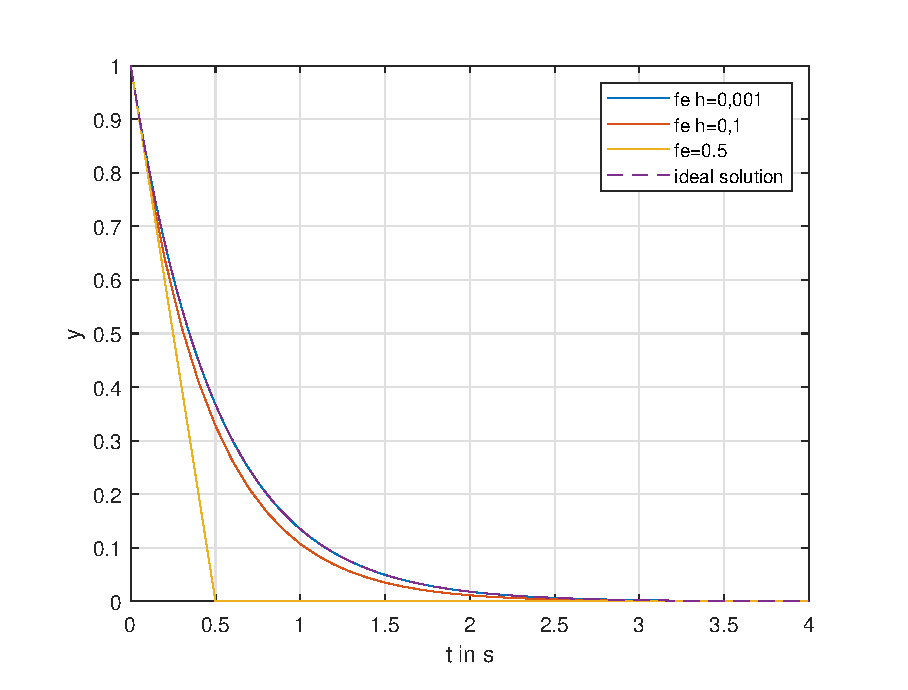
\includegraphics[width=\plotwidth]{plots/fe_only_equation_1.eps}
    \caption{Solution of Equation 1 with the Forward Euler algorithm}
    \label{fig:eq1_fe_only}
\end{figure}

\begin{figure}[H]
    \centering
    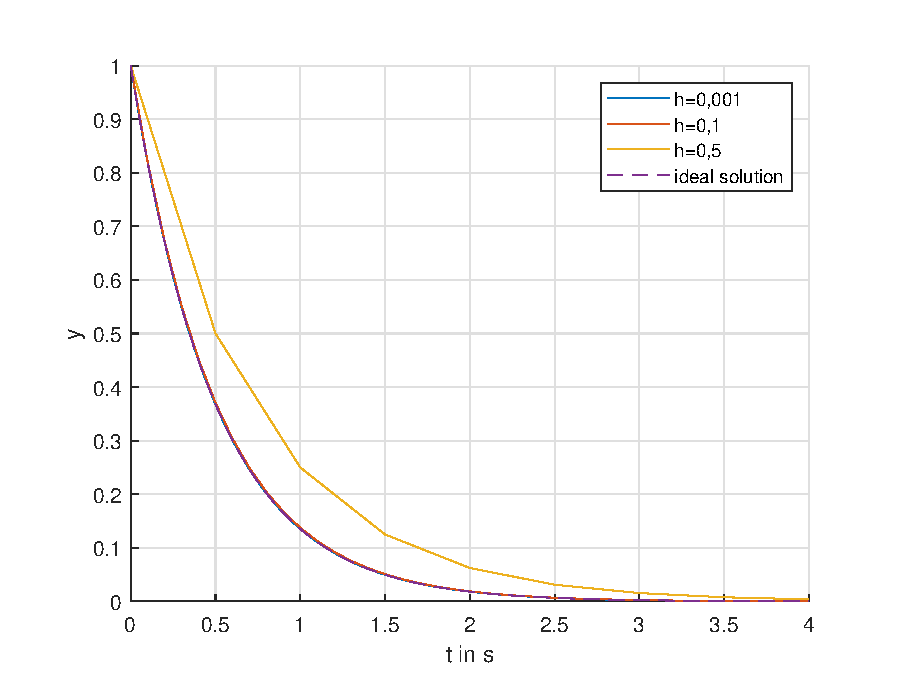
\includegraphics[width=\plotwidth]{plots/rk_only_equation_1.eps}
    \caption{Solution of Euqation 1 with the Midpoint algorithm}
    \label{fig:eq1_rk_only}
\end{figure}

%%%%%%%%%%%%%%%%%%%%%%%%%%%%%%%%%%%%%%%%%%%%%%%%%%%%%%%%%%%%%%%%%%%%%%%%%%%%%%%%%%%%%%%%%%%%%%%%%%%%%%%%%%%%%%%%%%%%%%%%%%
\section{equation 2}
\begin{figure}[H]
    \centering
    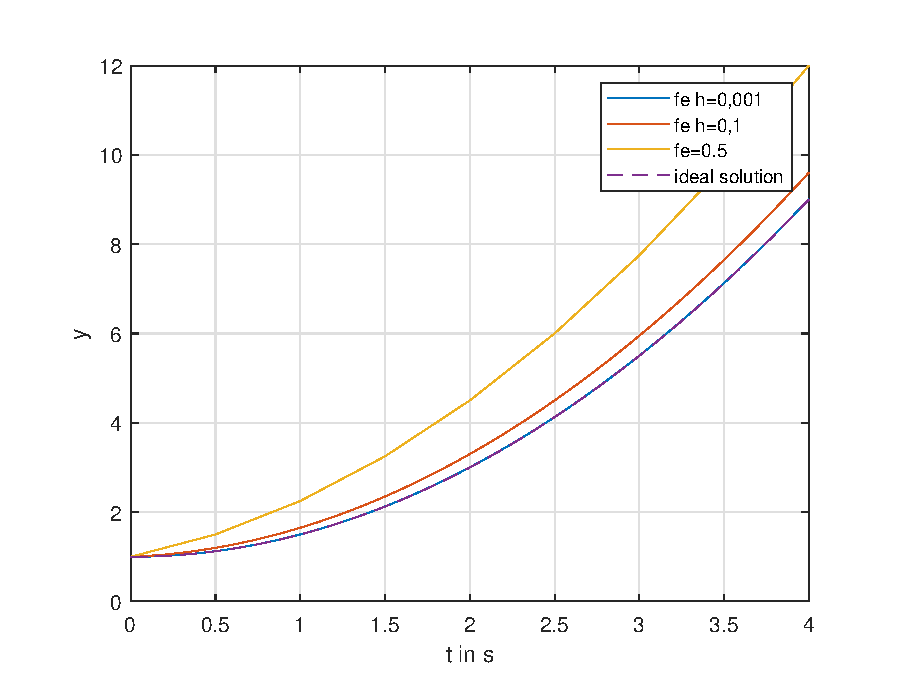
\includegraphics[width=\plotwidth]{plots/fe_only_equation_2.eps}
    \caption{Solution of Equation 2 with the Forward Euler algorithm}
    \label{fig:eq2_fe_only}
\end{figure}

\begin{figure}[H]
    \centering
    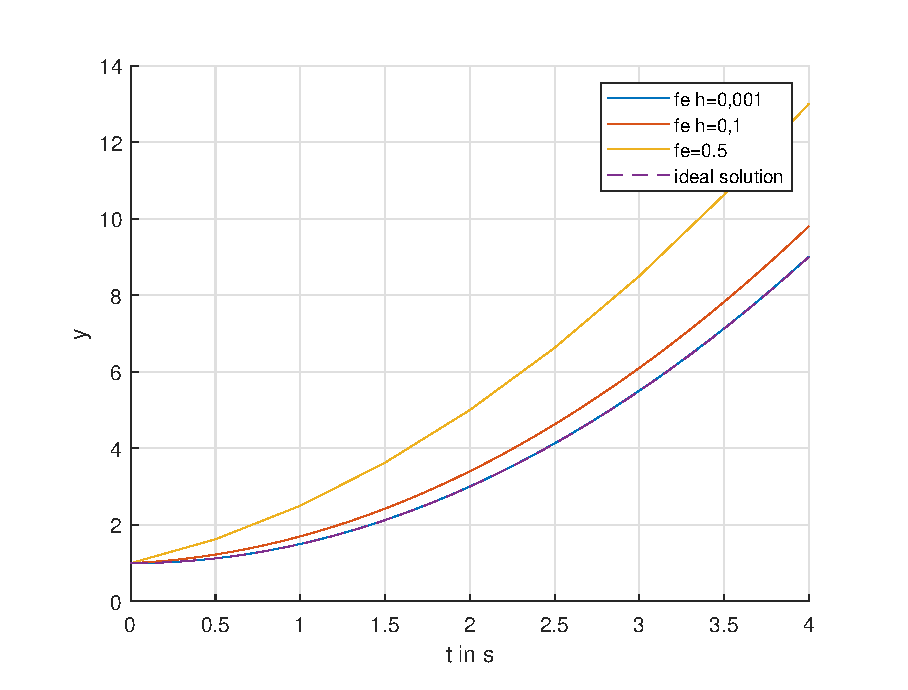
\includegraphics[width=\plotwidth]{plots/rk_only_equation_2.eps}
    \caption{Solution of Equation 2 with the Midpoint algorithm}
    \label{fig:eq2_rk_only}
\end{figure}
\begin{figure}[H]
    \centering
    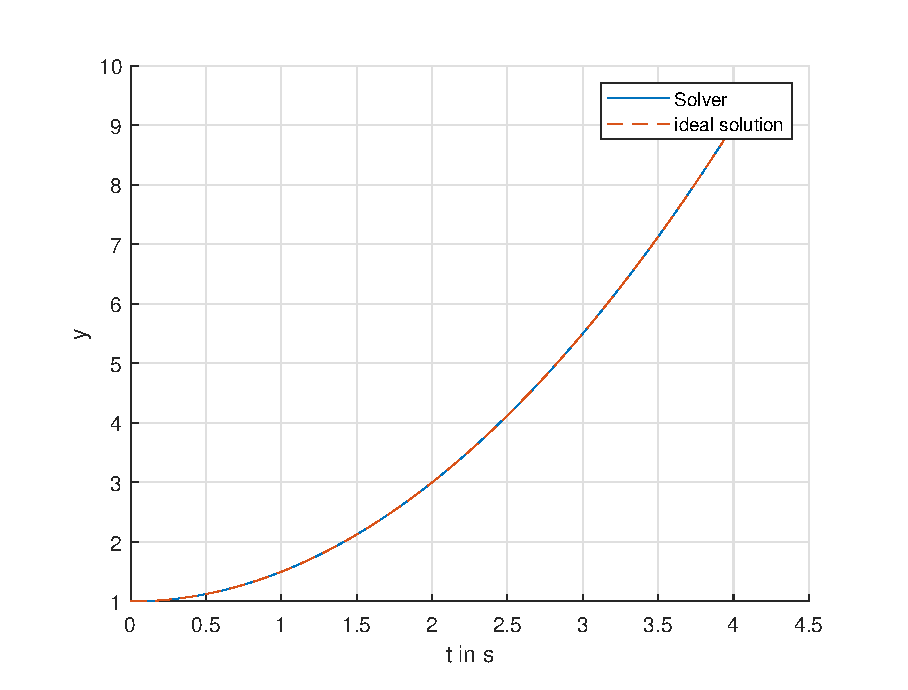
\includegraphics[width=\plotwidth]{plots/vs_only_equation_2.eps}
    \caption{Solution of Equation 2 with the Midpoint algorithm}
    \label{fig:eq2_rk_only}
\end{figure}

%%%%%%%%%%%%%%%%%%%%%%%%%%%%%%%%%%%%%%%%%%%%%%%%%%%%%%%%%%%%%%%%%%%%%%%%%%%%%%%%%%%%%%%%%%%%%%%%%%%%%%%%%%%%%%%%%%%%%%%%%%
\section{equation 2}
\begin{figure}[H]
    \centering
    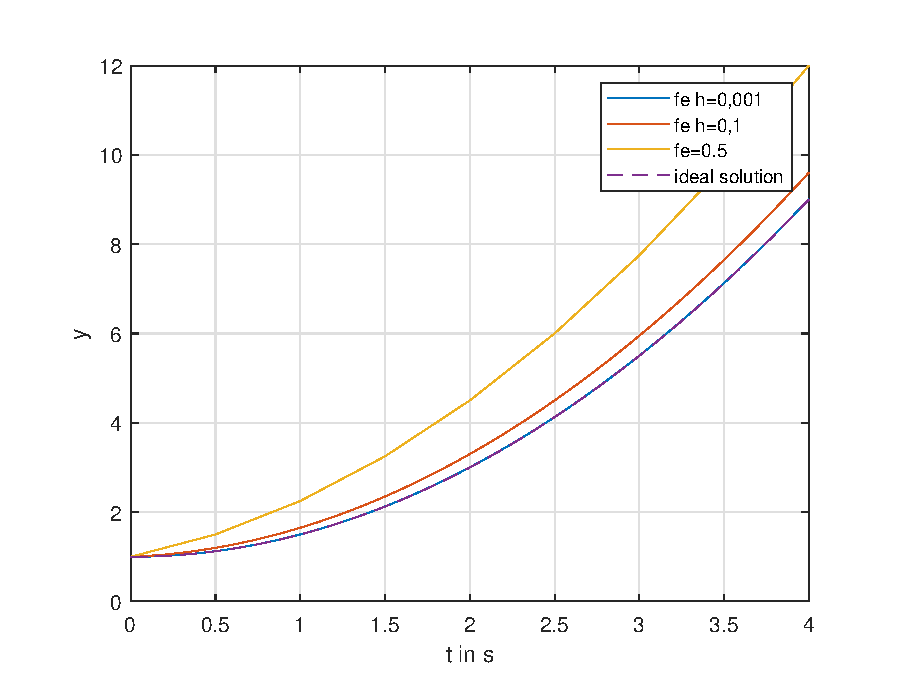
\includegraphics[width=\plotwidth]{plots/fe_only_equation_2.eps}
    \caption{Solution of Equation 2 with the Forward Euler algorithm}
    \label{fig:eq2_fe_only}
\end{figure}

\begin{figure}[H]
    \centering
    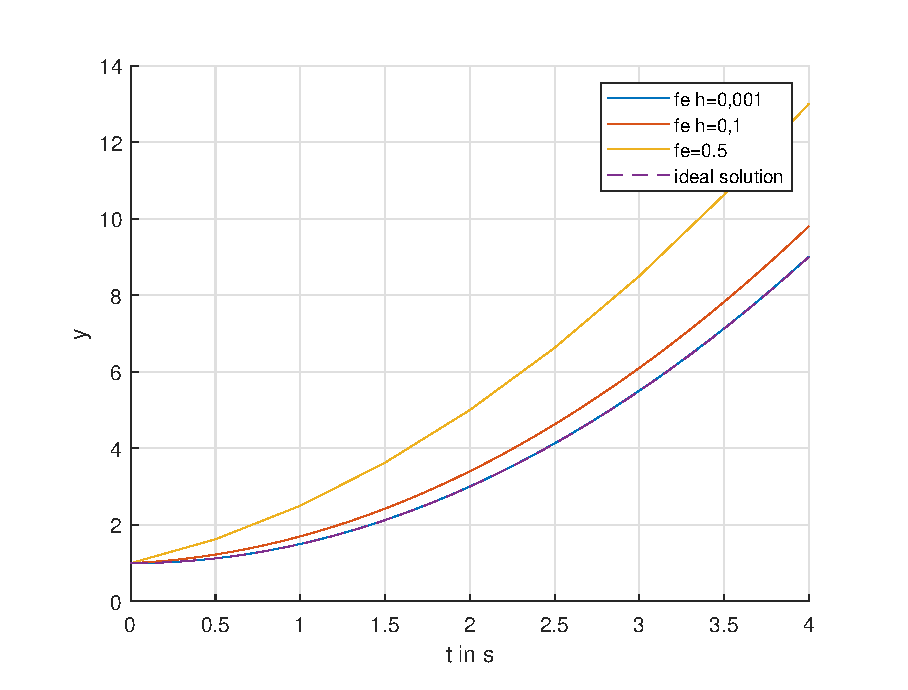
\includegraphics[width=\plotwidth]{plots/rk_only_equation_2.eps}
    \caption{Solution of Euqation 2 with the Midpoint algorithm}
    \label{fig:eq2_rk_only}
\end{figure}

%%%%%%%%%%%%%%%%%%%%%%%%%%%%%%%%%%%%%%%%%%%%%%%%%%%%%%%%%%%%%%%%%%%%%%%%%%%%%%%%%%%%%%%%%%%%%%%%%%%%%%%%%%%%%%%%%%%%%%%%%%
\section{equation 3}
\begin{figure}[H]
    \centering
    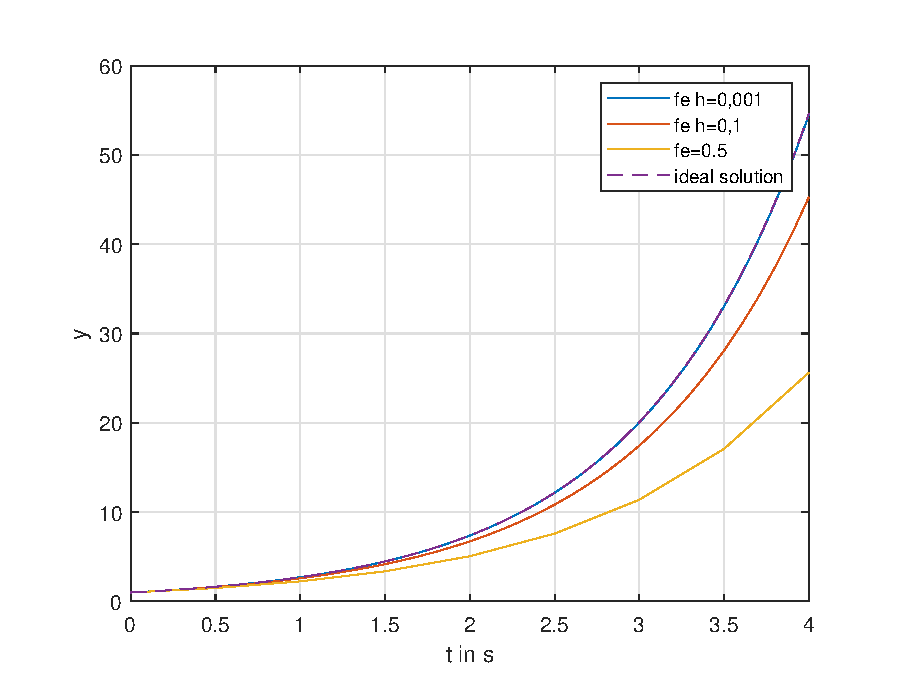
\includegraphics[width=\plotwidth]{plots/fe_only_equation_3.eps}
    \caption{Solution of Equation 3 with the Forward Euler algorithm}
    \label{fig:eq3_fe_only}
\end{figure}

\begin{figure}[H]
    \centering
    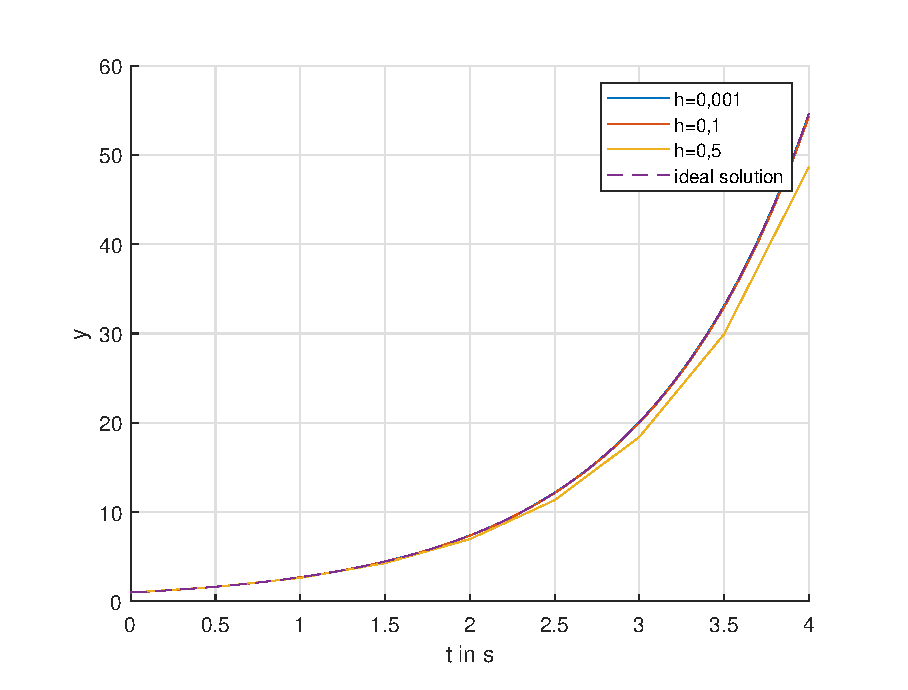
\includegraphics[width=\plotwidth]{plots/rk_only_equation_3.eps}
    \caption{Solution of Euqation 3 with the Midpoint algorithm}
    \label{fig:eq3_rk_only}
\end{figure}

%%%%%%%%%%%%%%%%%%%%%%%%%%%%%%%%%%%%%%%%%%%%%%%%%%%%%%%%%%%%%%%%%%%%%%%%%%%%%%%%%%%%%%%%%%%%%%%%%%%%%%%%%%%%%%%%%%%%%%%%%%
\section{equation 4}
\begin{figure}[H]
    \centering
    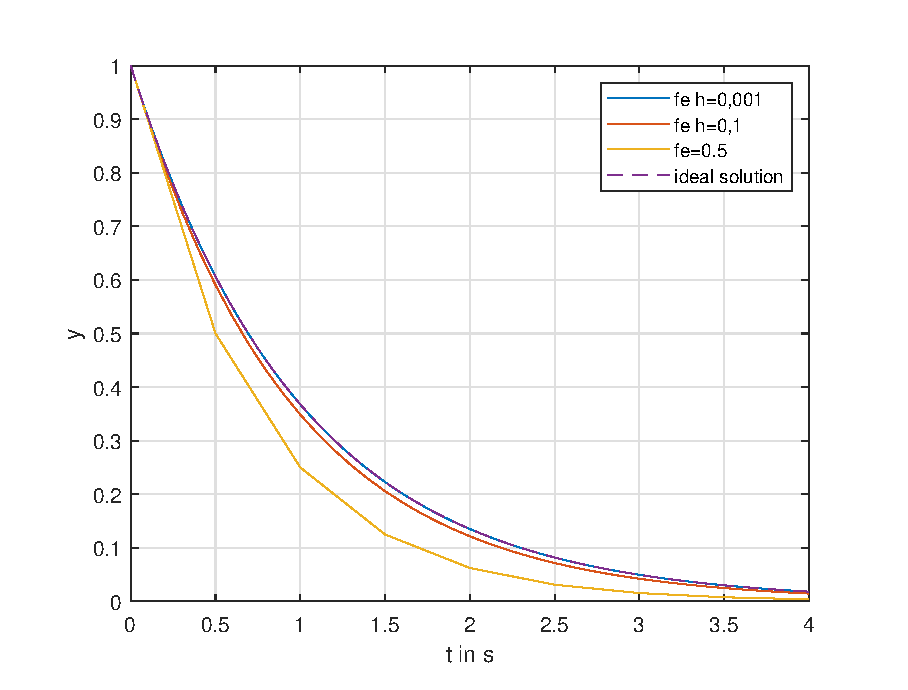
\includegraphics[width=\plotwidth]{plots/fe_only_equation_4.eps}
    \caption{Solution of Equation 4 with the Forward Euler algorithm}
    \label{fig:eq4_fe_only}
\end{figure}

\begin{figure}[H]
    \centering
    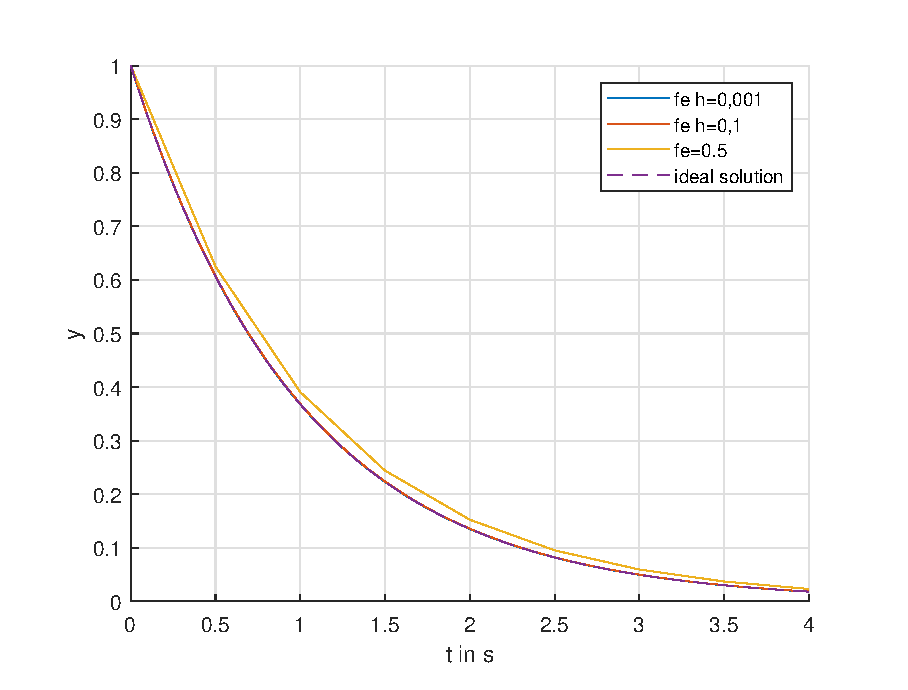
\includegraphics[width=\plotwidth]{plots/rk_only_equation_4.eps}
    \caption{Solution of Euqation 4 with the Midpoint algorithm}
    \label{fig:eq4_rk_only}
\end{figure}

%%%%%%%%%%%%%%%%%%%%%%%%%%%%%%%%%%%%%%%%%%%%%%%%%%%%%%%%%%%%%%%%%%%%%%%%%%%%%%%%%%%%%%%%%%%%%%%%%%%%%%%%%%%%%%%%%%%%%%%%%%
\section{equation 5}
\begin{figure}[H]
    \centering
    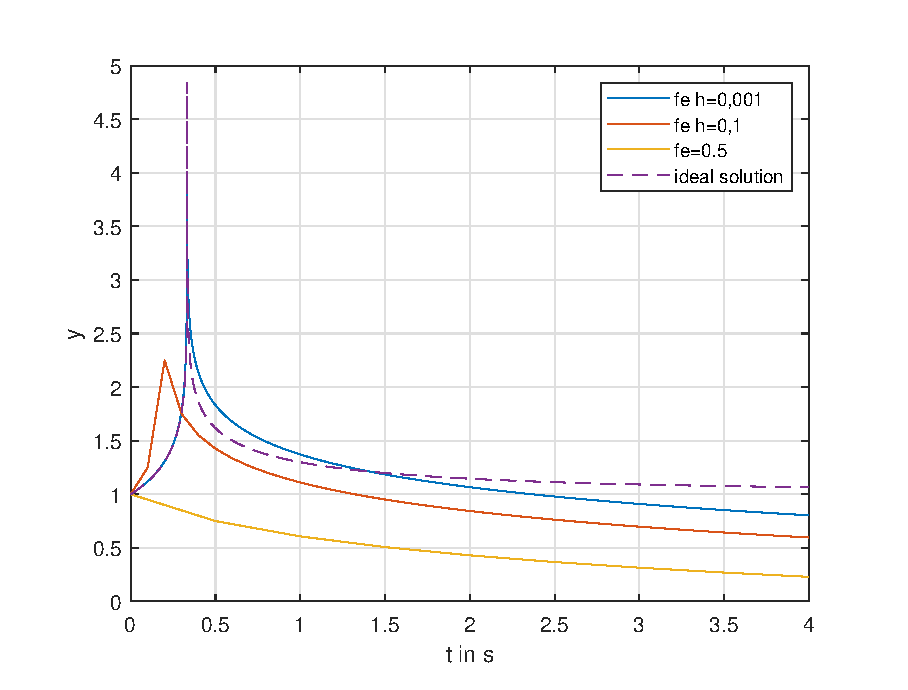
\includegraphics[width=\plotwidth]{plots/fe_only_equation_5.eps}
    \caption{Solution of Equation 5 with the Forward Euler algorithm}
    \label{fig:eq5_fe_only}
\end{figure}

\begin{figure}[H]
    \centering
    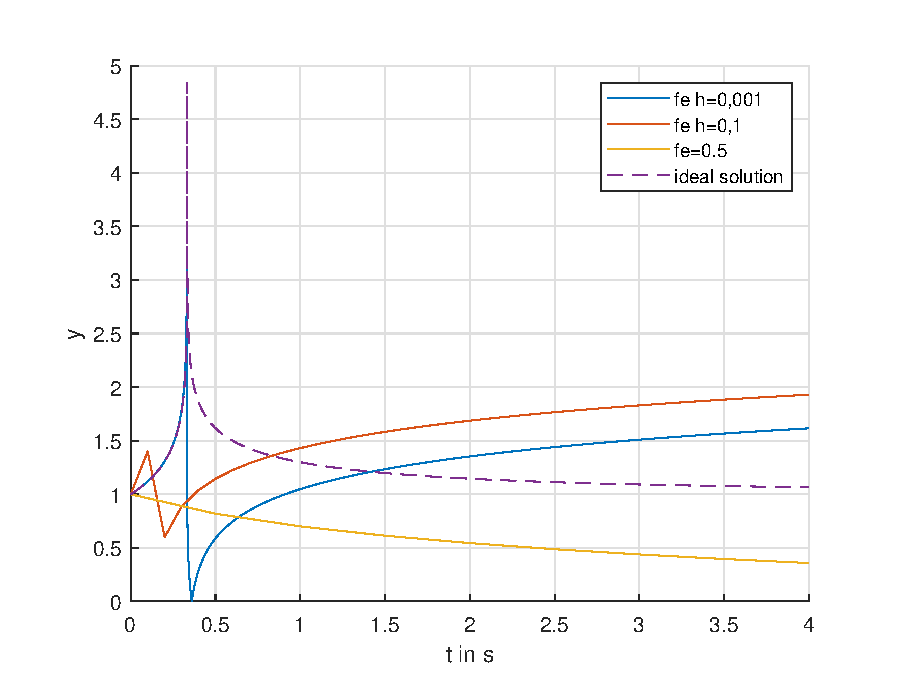
\includegraphics[width=\plotwidth]{plots/rk_only_equation_5.eps}
    \caption{Solution of Euqation 5 with the Midpoint algorithm}
    \label{fig:eq5_rk_only}
\end{figure}

%%%%%%%%%%%%%%%%%%%%%%%%%%%%%%%%%%%%%%%%%%%%%%%%%%%%%%%%%%%%%%%%%%%%%%%%%%%%%%%%%%%%%%%%%%%%%%%%%%%%%%%%%%%%%%%%%%%%%%%%%%
\section{equation 6}
\begin{figure}[H]
    \centering
    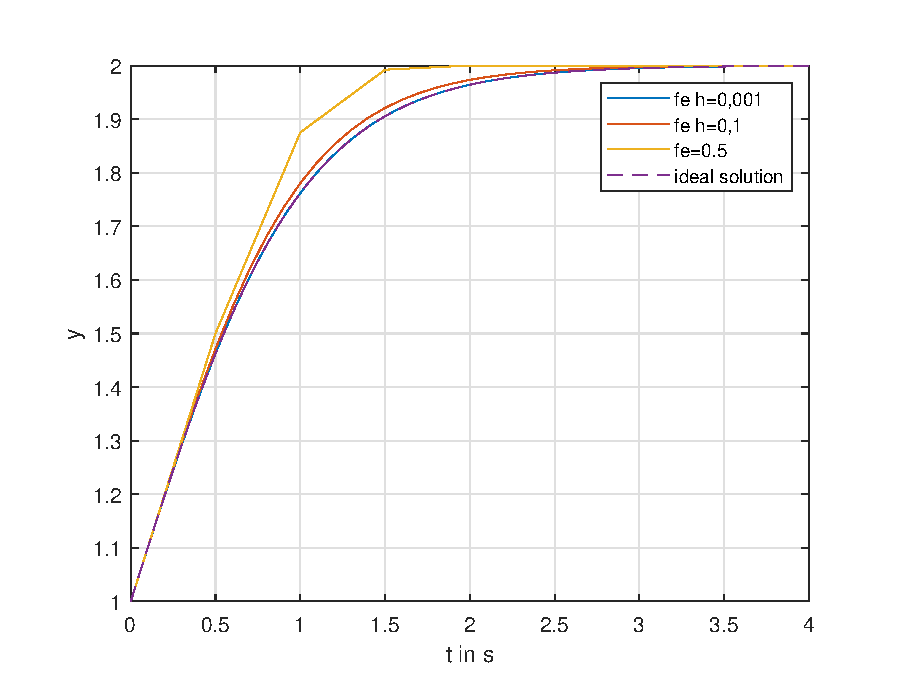
\includegraphics[width=\plotwidth]{plots/fe_only_equation_6.eps}
    \caption{Solution of Equation 6 with the Forward Euler algorithm}
    \label{fig:eq6_fe_only}
\end{figure}

\begin{figure}[H]
    \centering
    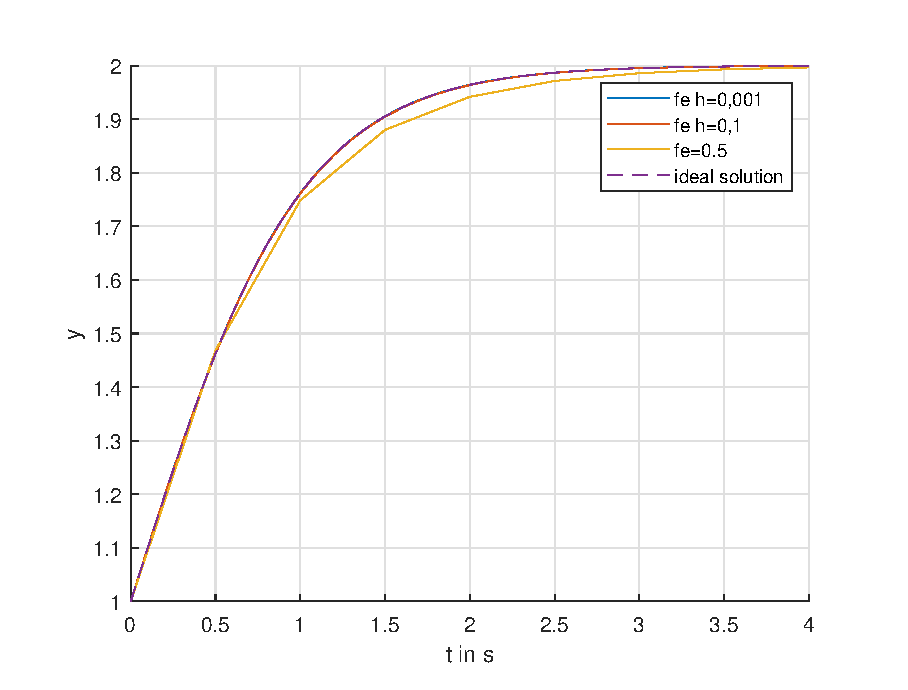
\includegraphics[width=\plotwidth]{plots/rk_only_equation_6.eps}
    \caption{Solution of Euqation 6 with the Midpoint algorithm}
    \label{fig:eq6_rk_only}
\end{figure}

\newpage
\chapter{Signaturen}
    Fertig gestellt am \today \\
    \begin{figure}[H]
        \centering
        
\includegraphics{pics/signature_grebien.png}
    	\caption{Signatur: Grebien Alexander}
    	\label{pic:signatur_grebien}
    \end{figure}
        
\listoffigures
\listoftables
\bibliographystyle{ieeetr}
\bibliography{meine_Zitatsbibliothek.bib}
\end{document}